%----------------
% Getting Started
%----------------

\section*{Getting started}
  \label{sec:getting-started}

  One of the main goals of scikit-image is to make it easy for any user to get started quickly--especially users already familiar with Python's scientific tools. To that end, the basic image is just a standard NumPy array, which exposes pixel data directly to the user. A new user can simply the load an image from disk (or use one of scikit-image's sample images), process that image with one or more image filters, and quickly display the results:

  % Bring in correctly syntax highlighted example
  \begin{pyverbatim}
    from skimage import data, io, filter

    image = data.coins()  # or any NumPy array!
    edges = filter.sobel(image)
    io.imshow(edges)
  \end{pyverbatim}

  \begin{figure}
    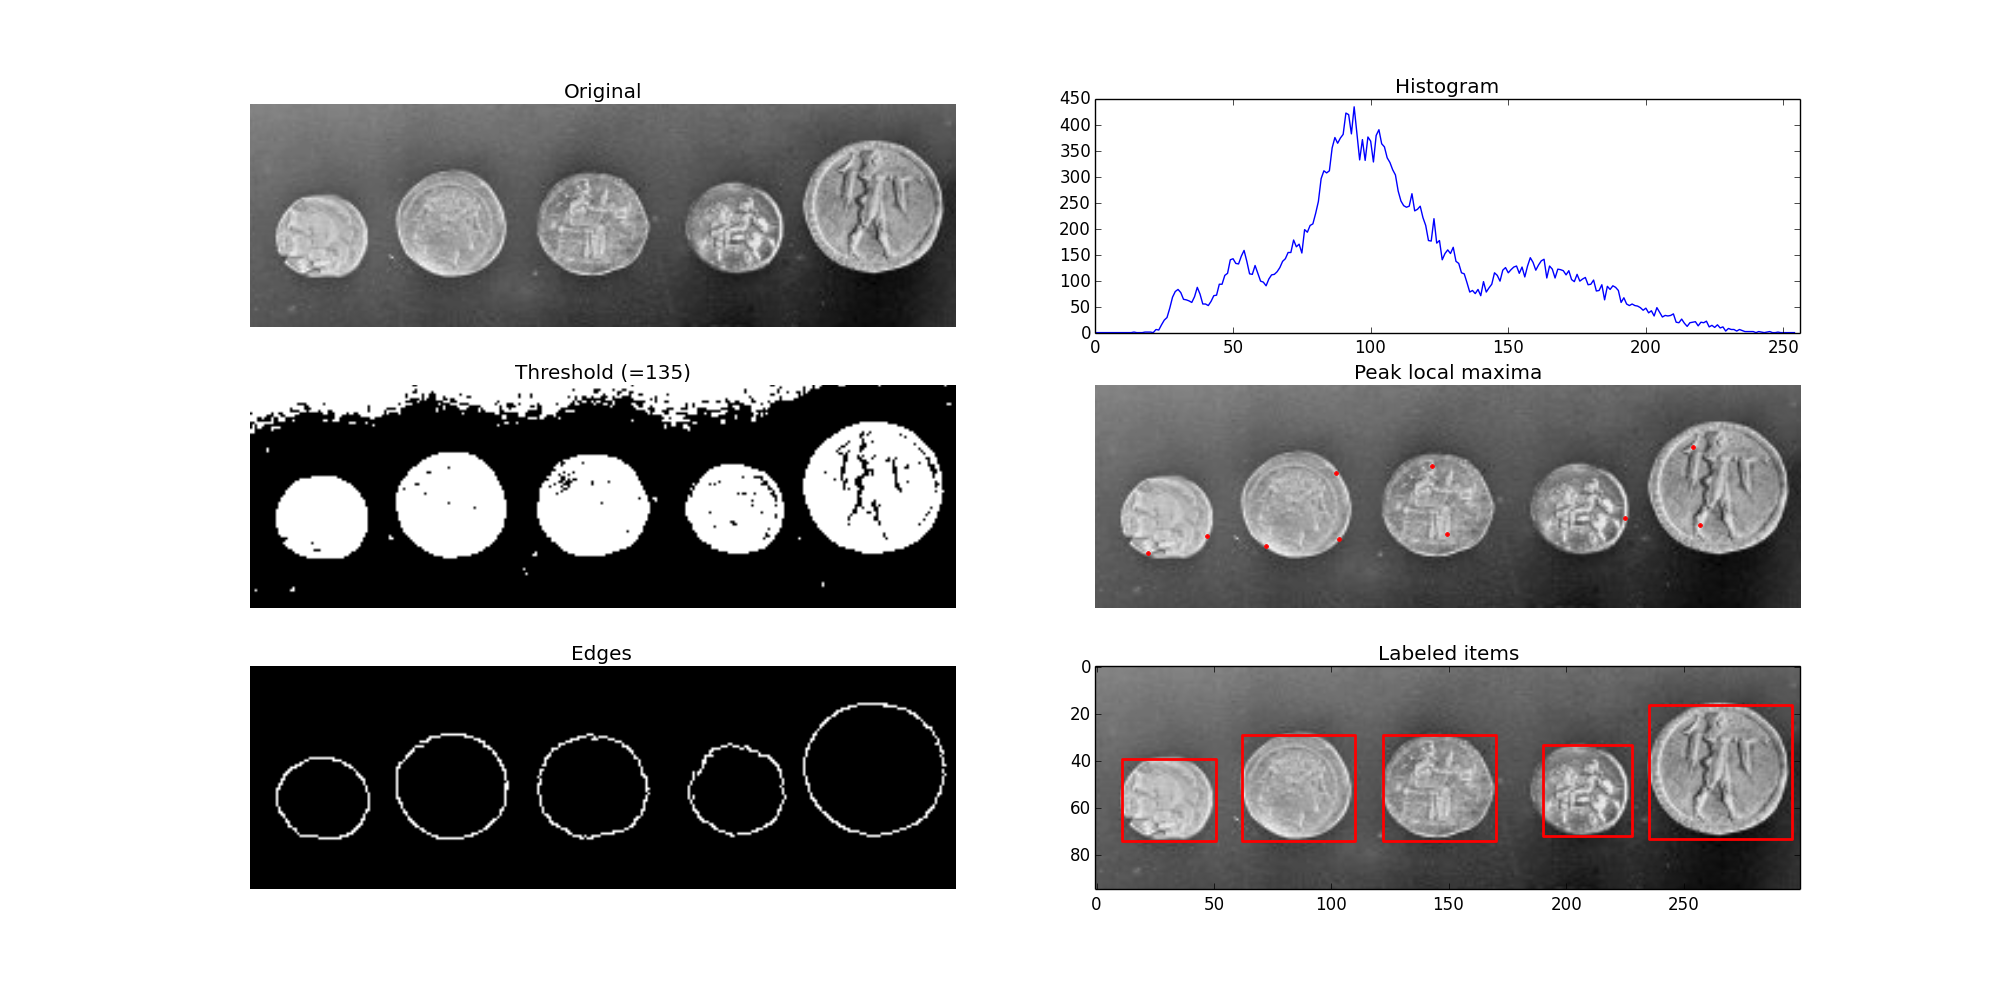
\includegraphics[width=\columnwidth]{getting_started}

    \caption[Getting started figure]{\label{fig:gettingstarted}Illustration of several functions available in scikit-image: adaptive threshold, local maxima, edge detection and labels. The use of NumPy arrays as our data container also enables the use of NumPy's built-in \texttt{histogram} function.}
  \end{figure}

  The above demonstration loads \texttt{data.coins}, an example image shipped with scikit-image.  For a more complete example, we import NumPy for array manipulation and matplotlib for plotting \citep{numpy,matplotlib}.  At each step, we add the picture or the plot to a matplotlib figure shown in Figure~\ref{fig:gettingstarted}.

  \begin{pyverbatim}
    import numpy as np
    import matplotlib.pyplot as plt

    # Load a small section of the image.
    image = data.coins()[0:95, 70:370]

    fig, axes = plt.subplots(ncols=2, nrows=3,
                             figsize=(8, 4))
    ax0, ax1, ax2, ax3, ax4, ax5  = axes.flat
    ax0.imshow(image, cmap=plt.cm.gray)
    ax0.set_title('Original', fontsize=24)
    ax0.axis('off')
  \end{pyverbatim}

  Since the image is represented by a NumPy array, we can easily perform operations such as building an histogram of the intensity values.

  \begin{pyverbatim}
    # Histogram.
    values, bins = np.histogram(image,
                                bins=np.arange(256))

    ax1.plot(bins[:-1], values, lw=2, c='k')
    ax1.set_xlim(xmax=256)
    ax1.set_yticks([0, 400])
    ax1.set_aspect(.2)
    ax1.set_title('Histogram', fontsize=24)
  \end{pyverbatim}

  To divide the foreground and background, we threshold the image to produce a binary image.  Several threshold algorithms are available. Here, we employ \linebreak\texttt{filter.threshold\_adaptive} where the threshold value is the weighted mean for the local neighborhood of a pixel.

  \begin{pyverbatim}
    # Apply threshold.
    from skimage.filter import threshold_adaptive

    bw = threshold_adaptive(image, 95, offset=-15)

    ax2.imshow(bw, cmap=plt.cm.gray)
    ax2.set_title('Adaptive threshold', fontsize=24)
    ax2.axis('off')
  \end{pyverbatim}

  We can easily detect interesting features, such as local maxima and edges. The function \texttt{feature.peak\_local\_max} can be used to return the coordinates of local maxima in an image.

  \begin{pyverbatim}
    # Find maxima.
    from skimage.feature import peak_local_max

    coordinates = peak_local_max(image, min_distance=20)

    ax3.imshow(image, cmap=plt.cm.gray)
    ax3.autoscale(False)
    ax3.plot(coordinates[:, 1],
             coordinates[:, 0], c='r.')
    ax3.set_title('Peak local maxima', fontsize=24)
    ax3.axis('off')
  \end{pyverbatim}

  Next, a Canny filter (\texttt{filter.canny}) \citep{Canny} detects the edge of each coin.

  \begin{pyverbatim}
    # Detect edges.
    from skimage import filter

    edges = filter.canny(image, sigma=3,
                         low_threshold=10,
                         high_threshold=80)

    ax4.imshow(edges, cmap=plt.cm.gray)
    ax4.set_title('Edges', fontsize=24)
    ax4.axis('off')
  \end{pyverbatim}

  Then, we attribute to each coin a label (\texttt{morphology.label}) that can be used to extract a sub-picture. Finally, physical information such as the position, area, eccentricity, perimeter, and moments can be extracted using \texttt{measure.regionprops}.

  \begin{pyverbatim}
    # Label image regions.
    from skimage.measure import regionprops
    import matplotlib.patches as mpatches
    from skimage.morphology import label

    label_image = label(edges)

    ax5.imshow(image, cmap=plt.cm.gray)
    ax5.set_title('Labeled items', fontsize=24)
    ax5.axis('off')

    for region in regionprops(label_image):
        # Draw rectangle around segmented coins.
        minr, minc, maxr, maxc = region.bbox
        rect = mpatches.Rectangle((minc, minr),
                                  maxc - minc,
                                  maxr - minr,
                                  fill=False,
                                  edgecolor='red',
                                  linewidth=2)
        ax5.add_patch(rect)

    plt.tight_layout()
    plt.show()
  \end{pyverbatim}

  scikit-image thus makes it possible to perform sophisticated image processing tasks with only a few function calls.
